\documentclass[uplatex,dvipdfmx,a4paper,11pt]{jsarticle}

\usepackage[top=25mm,bottom=25mm,left=25mm,right=25mm]{geometry}
\usepackage{array}
\usepackage{tabularx}
\usepackage{booktabs}
\usepackage{enumitem}
\usepackage{graphicx}

\setlength{\parindent}{0pt}
\setlength{\parskip}{0.6em}

\usepackage{titlesec}
\titleformat{\section}
  {\normalfont\Large\bfseries}{\thesection.}{0.6em}{}
\titleformat{\subsection}
  {\normalfont\large\bfseries}{\thesubsection}{0.6em}{}
\titlespacing*{\section}{0pt}{1.2em}{0.6em}
\titlespacing*{\subsection}{0pt}{1.0em}{0.4em}

\newcommand{\sectionrule}{\par\medskip\noindent\rule{\linewidth}{0.6pt}\par\medskip}

\renewcommand{\labelitemi}{\textbullet}
\renewcommand{\labelitemii}{\textopenbullet}
\setlist[itemize]{leftmargin=1.6em,itemsep=0.1em,topsep=0.2em}
\setlist[enumerate]{leftmargin=2.0em,itemsep=0.1em,topsep=0.2em}

\providecommand{\textopenbullet}{\ensuremath{\circ}}

\begin{document}

{\LARGE\bfseries 作業ログ}\par\bigskip

報告者：梅澤颯太

報告日：2026年6月16日

プロジェクト名：タクトーン～IMU ジェスチャーで奏でるArduino オーケストラ～

\sectionrule

\section{進捗サマリー（要約）}

\begin{itemize}
  \item 全体進捗率：95\%
  \item マイルストーン達成状況：ガントチャートに載っている個人のタスクは全て完了
  \item 主要成果：
    \begin{itemize}
      \item 指揮棒側を3Dプリンタで作成するため，3Dモデリングソフトの操作練習を行った．
      \item MOP検証方法について，既存の目標値に対してどのような手順で確認するかを検討した．
    \end{itemize}
  \item 課題：
    \begin{itemize}
      \item 指揮棒側の形状はまだ練習段階であり，さらに実際の部品寸法を検討する必要がある．
      \item MOP検証方法は検討を始めた段階であり，実機で測定する項目と記録方法を具体化する必要がある．
    \end{itemize}
\end{itemize}

\subsection{ガントチャート}

\begin{figure}[htbp]
  \centering
  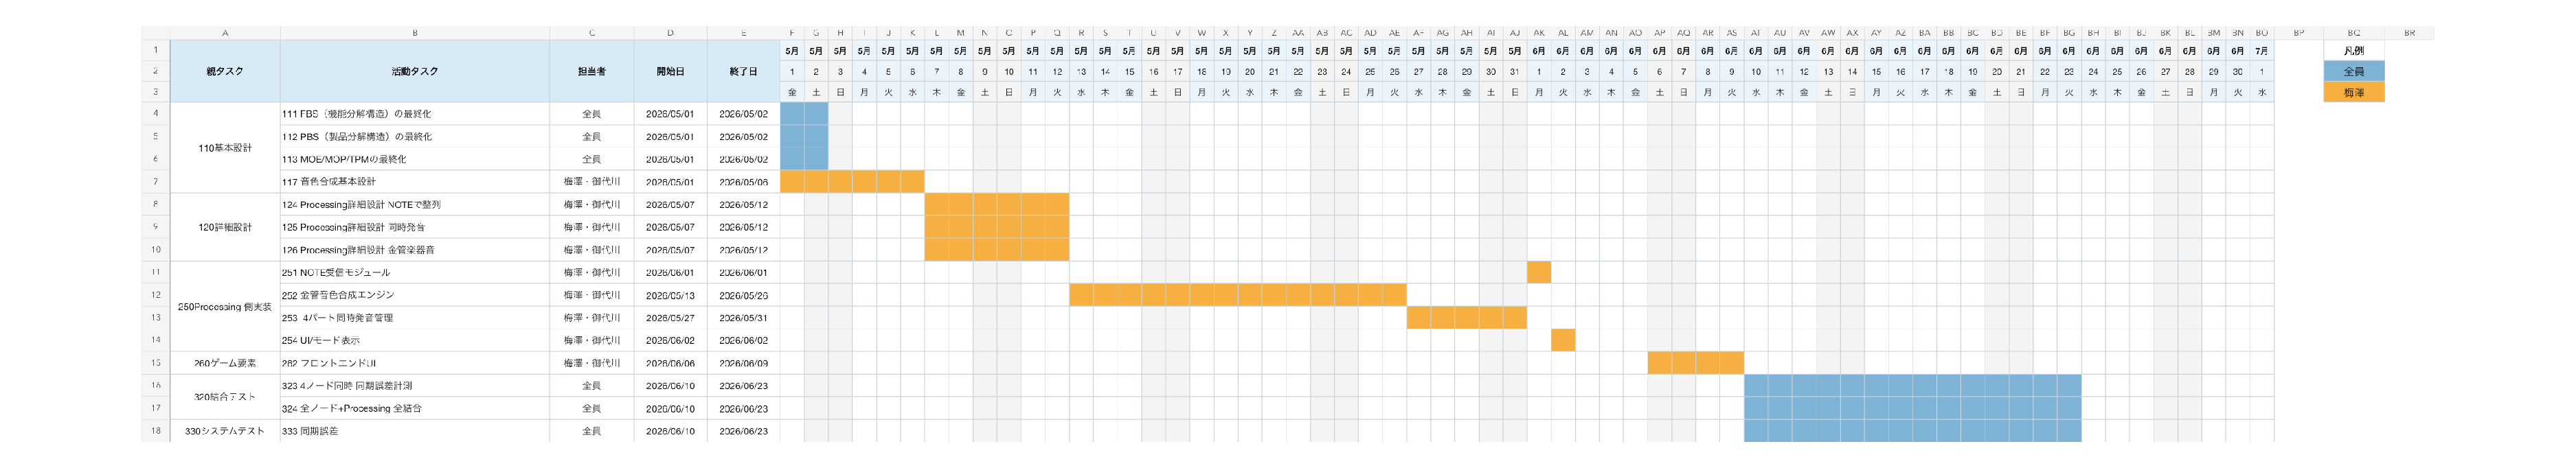
\includegraphics[width=\linewidth]{fig/ガントチャート_梅澤_全員.pdf}
  \caption{全体のガントチャート}
\end{figure}

\sectionrule

\section{作業ログ（詳細トラッキング）}

\begin{tabularx}{\linewidth}{@{}p{0.16\linewidth}p{0.12\linewidth}XX@{}}
\toprule
日付 & 作業時間 & 作業内容 & 成果・メモ \\
\midrule
2026/06/14 & 1.5h & 指揮棒側を3Dプリンタで作るためのモデリング練習を行った． & 3Dモデリングソフトの基本操作を確認し，指揮棒側の外装や保持部を作るために必要な形状作成の流れを練習した． \\
2026/06/16 & 10min & MOP検証方法の検討を行った． & 同期誤差，通信遅延，拍検出精度などのMOPについて，実機で確認する際にどのような測定項目が必要かを整理した． \\
\bottomrule
\end{tabularx}

\sectionrule

%================================================================
% 3. 課題管理
%================================================================
\section{課題管理}

\begin{tabularx}{\linewidth}{@{}p{0.20\linewidth}Xp{0.08\linewidth}p{0.08\linewidth}Xp{0.11\linewidth}p{0.09\linewidth}@{}}
\toprule
課題 & 発生原因 & 影響度 & 優先度 & 対策 & 期限 & 状態 \\
\midrule
指揮棒側モデルの具体化 & 今回はモデリング練習が中心であり，実際に3Dプリンタで出力するモデルまでは作成していない． & 中 & 中 & 実際に使う部品の寸法を確認し，持ちやすさと内部スペースを考慮したモデルを作成する． & 次回以降 & 対応予定 \\
MOP検証方法の具体化 & 今回は検証方法の検討にとどまり，実機での測定手順や記録形式までは確定していない． & 中 & 中 & MOPごとに測定対象，使用機材，記録項目，合否基準を表に整理する． & 実機検証前 & 対応中 \\
\bottomrule
\end{tabularx}

\sectionrule

%================================================================
% 4. AI利用状況と検証
%================================================================
\section{AI利用状況と検証（再現性重視）}

\subsection{利用内容}

\begin{itemize}
  \item 利用目的：作業ログ文章の作成補助，MOP検証方法の整理補助
  \item 入力（プロンプト要旨）：
    \begin{itemize}
      \item 以前の作業ログを参考に今週分の作業ログを作成するよう依頼した．
      \item 今週の作業として，指揮棒側を3Dプリンタで作るためのモデリング練習を1時間半行ったこと，MOP検証方法を10分程度検討したことを伝えた．
    \end{itemize}
  \item 出力概要：
    \begin{itemize}
      \item 以前の作業ログ形式に合わせて，進捗サマリー，作業ログ，課題管理，AI利用状況，次回計画の文章を作成した．
      \item ガントチャート上の個人のタスクが完了していることと，今週行った追加作業を分けて整理できた．
    \end{itemize}
\end{itemize}

\sectionrule

\subsection{検証方法}

\begin{itemize}
  \item 検証手法：
    \begin{itemize}
      \item 作業ログの内容が実際の作業内容と一致しているかを確認する．
    \end{itemize}
  \item 検証手順：
    \begin{enumerate}
      \item 生成されたものを実際の作業内容と照らし合わせる．
    \end{enumerate}
\end{itemize}

\sectionrule

\subsection{ファクトチェック結果}

\begin{itemize}
  \item 一致点：
    \begin{itemize}
      \item 記載されていることは全て一致していた．
    \end{itemize}
  \item 不一致・疑義：
    \begin{itemize}
      \item なし
    \end{itemize}
  \item 最終判断：
    \begin{itemize}
      \item レポート本文として採用する．
    \end{itemize}
  \item 根拠：
    \begin{itemize}
      \item 実際の作業内容を正確に反映しているため．
    \end{itemize}
\end{itemize}

\sectionrule

%================================================================
% 5. 次回計画
%================================================================
\section{次回計画}

\begin{itemize}
  \item 目標：
    \begin{itemize}
      \item 指揮棒側の3Dプリンタ出力に向けて，実際の部品寸法を反映したモデルを作成する．
      \item MOP検証を，実機で実行できるようにする．
    \end{itemize}
  \item 達成基準：
    \begin{itemize}
      \item 指揮棒側モデルについて，指揮棒として違和感のない形になっていること．
      \item MOP検証に基づいて，実機での測定項目と記録方法が確定していること．
    \end{itemize}
  \item 期限：
    \begin{itemize}
      \item 次回作業時
    \end{itemize}
\end{itemize}

\sectionrule

%================================================================
% 6. その他
%================================================================
\section{その他}

\begin{itemize}
  \item ガントチャートに載っているタスクは完了したため，今週は発表に向けた外装検討と検証方法の整理を行った．
  \item 3Dプリンタで指揮棒側を作る場合，電子部品の寸法だけでなく，配線の逃げや持ったときの安定性も考慮する必要がある．
\end{itemize}

\sectionrule

%================================================================
% 7. 付録
%================================================================
\section{付録}

無し

\sectionrule

\end{document}
